\documentclass[../main.tex]{subfiles}
\begin{document}
\chapter{Editor Features}
\label{chapter:editor-featres}
% \todo[inline]{This section needs updating. The screenshots should be replaced with screenshots using the default colour scheme. There needs to be examples of higher-order predicates.}
The Logical English editor provides various features that help the user understand, write, and correct Logical English. 
\section{Highlighting}
\begin{figure}[h!]
\centering
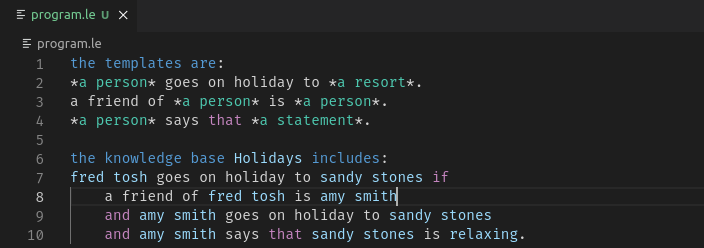
\includegraphics[width = \linewidth]{./figures/highlighting.png}
\caption{The editor highlighting grammatical components of a short Logical English program.}
\label{fig:highlighting}
\end{figure}
Figure \ref{fig:highlighting} shows the editor highlighting grammatical features of Logical English. The editor highlights 
\begin{itemize}
    \item titles of sections
    \item template variable names
    \item logical connectives between atomic formulas, and
    \item terms in atomic formulas.
\end{itemize}
As shown on line 12 of Figure \ref{fig:highlighting}, the editor highlights terms in atomic formulas recursively. If a higher-order atomic formula contains another atomic formula, then its terms are also highlighted.
\\
\\
Figure \ref{fig:highlighting}, as well as subsequent screenshots, are taken using the built-in `Default Dark+' colour theme of Visual Studio Code . Features of Logical English are highlighted regardless of the colour theme used, with the only change being the colours that features are given.

\section{Code Completion}\begin{figure}[h!]
\centering
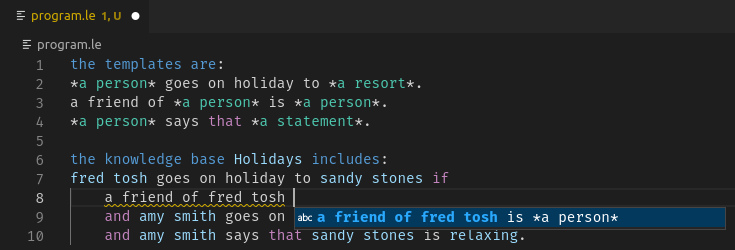
\includegraphics[width = \linewidth]{./figures/autocomplete.png}
\caption{The editor suggesting the remainder of an incomplete atomic formula.}
\label{fig:code-completion}
\end{figure}
Figure \ref{fig:code-completion} shows the editor suggesting the remainder of an incomplete atomic formula. This happens as the user is typing the atomic formula once the line the user is typing begins to conform to a template. When selecting the suggested formula, by clicking on the suggestion or pressing Tab, the suggested atomic formula is inserted with the remaining template arguments (such as `a person' in Figure \ref{fig:code-completion}) replaced by placeholders. The user can navigate across the placeholders by pressing Tab, allowing the user to fill in the placeholders efficiently.

\section{Error Diagnosis}
\section{Clauses with misaligned connectives}
\begin{figure}[h!]
\centering
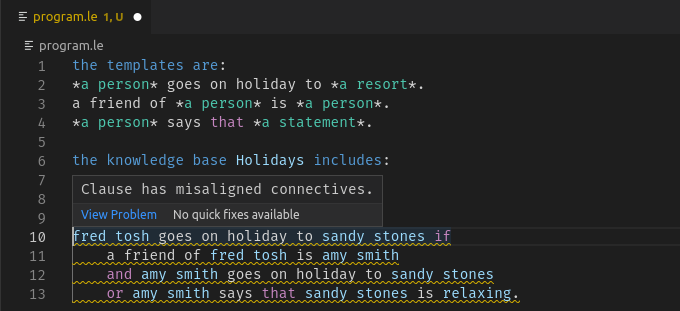
\includegraphics[width = \linewidth]{./figures/clause-misaligned-connectives.png}
\caption{The editor identifying a clause with misaligned connectives.}
\label{fig:misaligned-connectives}
\end{figure}
As shown in Figure  \ref{fig:misaligned-connectives}, the editor marks a clause with a warning when the clause has connectives whose order of precedence is not stated through indentation \footnote{This is discussed in section \ref{section:knowledge-base}}. On hovering over the clause, the editor produces the error message `Clause has misaligned connectives.'


\subsection{Atomic formulas without templates}
\label{section:no-template-feature}
\begin{figure}[h!]
\centering
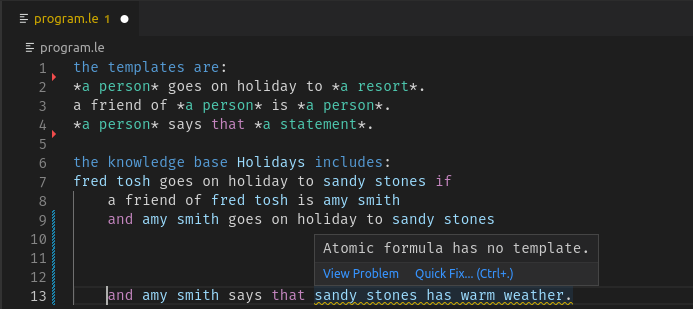
\includegraphics[width = \linewidth]{./figures/atomic-formula-no-template.png}
\caption{The editor identifying an atomic formula that does not match any of the templates.}
\label{fig:no-template-diag}
\end{figure}
As shown in Figure \ref{fig:no-template-diag}, if the document contains an atomic formula that does not conform to any template, the editor marks the atomic formula with an underline representing a warning. On hovering over the atomic formula, the editor produces an explanatory error message. 
% \\ 
% \\
% This feature occurs when an atomic formula does not conform to any template written in the document, nor any of Logical English's pre-defined templates.
\section{Code Actions}
% \begin{figure}[h!]
% \centering
% 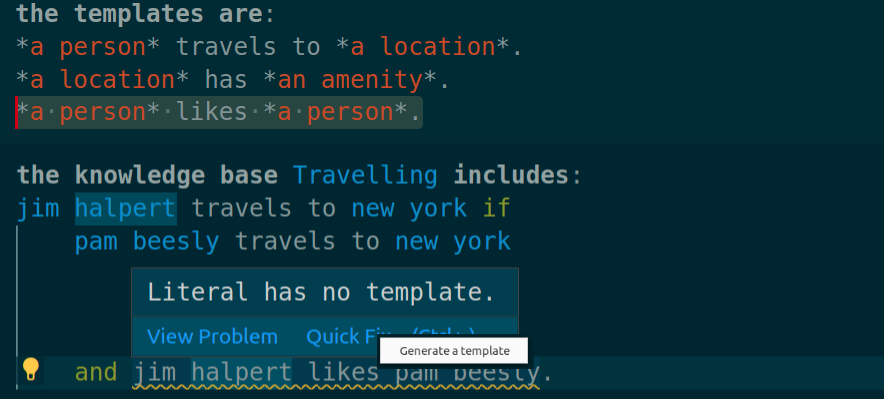
\includegraphics[width = \linewidth]{./figures/generate-template-full.png}
% \caption{The third template has been generated by the editor to match the underlined atomic formula.}
% \label{fig:new-template}
% \end{figure}
\begin{figure}%
    \centering
    \subfloat[\centering The document before the template is auto-generated.]{
        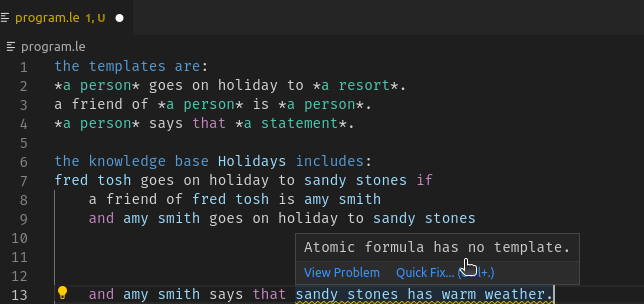
\includegraphics[width=0.9\linewidth]{figures/quickfix-before-croped.png} 
    }%
    % \qquad
    \\
    \subfloat[\centering The document after the template is auto-generated.]{
        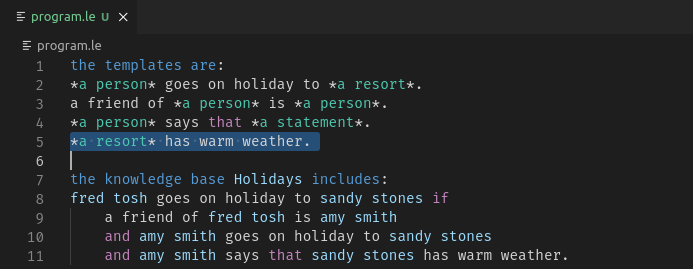
\includegraphics[width=0.9\linewidth]{figures/quickfix-after.png}
    }%
    \caption{2 Figures side by side}%
    \label{fig:new-template}%
\end{figure}
Figure \ref{fig:new-template} shows the process of generating a new template that conforms to atomic formulas. If a number of atomic formulas are marked as not conforming to any templates, hovering over any one of the atomic formulas produces an error message with the option `Quick Fix'. When selected, the editor auto-generates a single template that conforms to each atomic formula that was marked with this error. 
\\
\\
If the marked atomic formulas contain terms which also feature in atomic formulas that conform to templates, then the types of those terms will feature in the auto-generated template. This is shown in Figure \ref{fig:new-template}: the term \codeword{sandy stones} features in prior atomic formulas formulas and has type \codeword{a resort}. This allows the auto-generated template to feature the type \codeword{a resort}.

\section{Type Checking}
\subsection{Type Mismatch Errors}
\begin{figure}[h!]
\centering
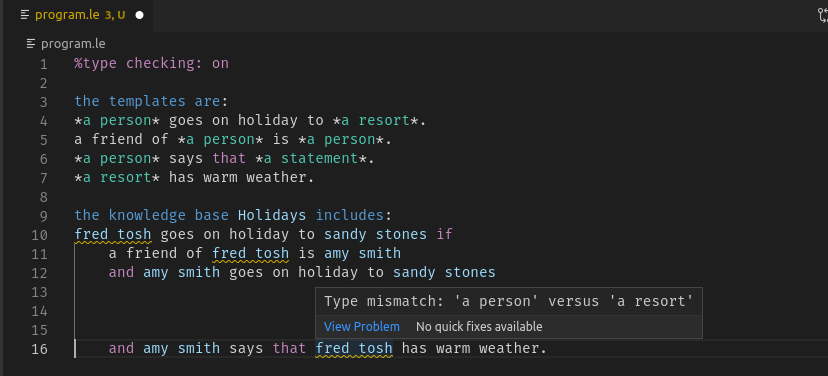
\includegraphics[width = \linewidth]{figures/type-error.png}
\caption{The editor identifying a type mismatch error.}
\label{fig:type-mismatch}
\end{figure}

The comment \codeword{%type checking: on}
(shown at the top of Figure \ref{fig:type-mismatch}) activates type checking features in the editor. If the following scenario occurs:
\begin{enumerate}
    \item an atomic formula contains a term $x$, where $x$ is assigned the type $A$
    \item another atomic formula in the same clause contains the same term $x$, where $x$ is assigned the type $B$
    \item $A$ and $B$ do not have the same name, nor is one a sub-type of the other (discussed in section \ref{section:type-hierarcy-features}).
\end{enumerate}
then all the instances of the term are marked as warnings. If any one of the terms are hovered over, a message appears that explains that there is a type mismatch between the two stated types.
\\
\\
This is demonstrated in Figure \ref{fig:type-mismatch}. The term \codeword{fred tosh} is assigned the type \codeword{a person} in the atomic formulas on line 10 and line 11, but is assigned the type \codeword{a resort} in the atomic formula on line 16. Since these two types are incompatible, an error message is produced.

\subsection{The Type Hierarchy}
\label{section:type-hierarcy-features}
% \begin{figure}[h!]
% \centering
% 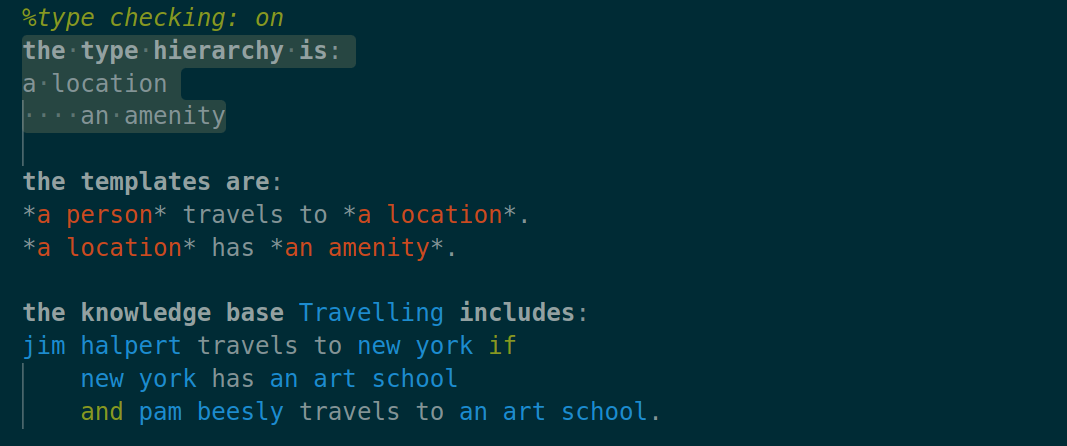
\includegraphics[width = \linewidth]{./figures/type-hierarchy.png}
% \caption{A type hierarchy that resolves the type mismatch error in Figure \ref{fig:type-mismatch}. The type \lstinline{a location} is now a subtype of \codeword{an amenity}.}
% \label{fig:type-hierarchy}
% \end{figure}
\begin{figure}%
    \centering
    \subfloat[\centering The editor marking the type mismatch error with the term \codeword{amy smith}.]{
        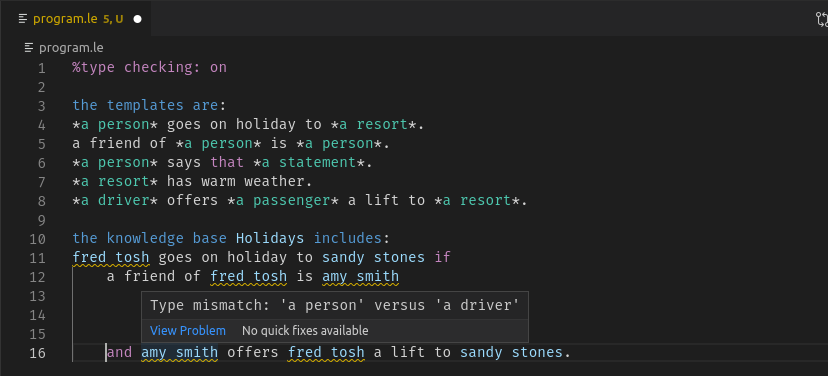
\includegraphics[width=0.9\linewidth]{figures/type-error-amy.png} 
    }%
    \\
    \subfloat[\centering The editor marking the type mismatch error with the term \codeword{fred tosh}.]{
        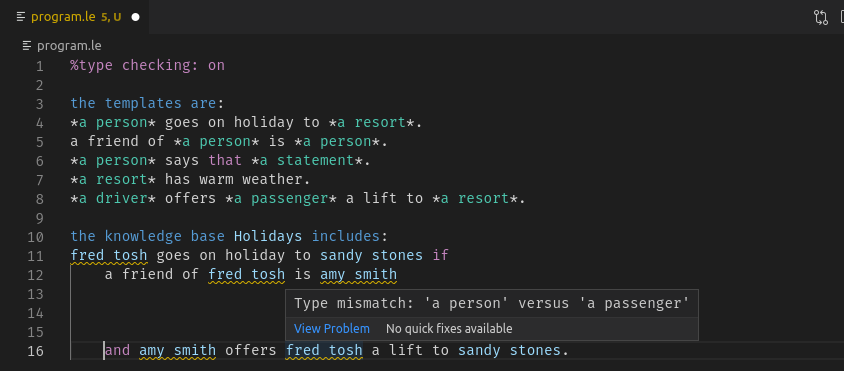
\includegraphics[width=0.9\linewidth]{figures/type-error-fred.png }
    }%
    \caption{The editor marking two type mismatch errors. The errors are caused by the types \codeword{a driver} and \codeword{a passenger} being incompatible with the type \codeword{a person}.}%
\label{fig:type-mismatch-2}
\end{figure}

\begin{figure}
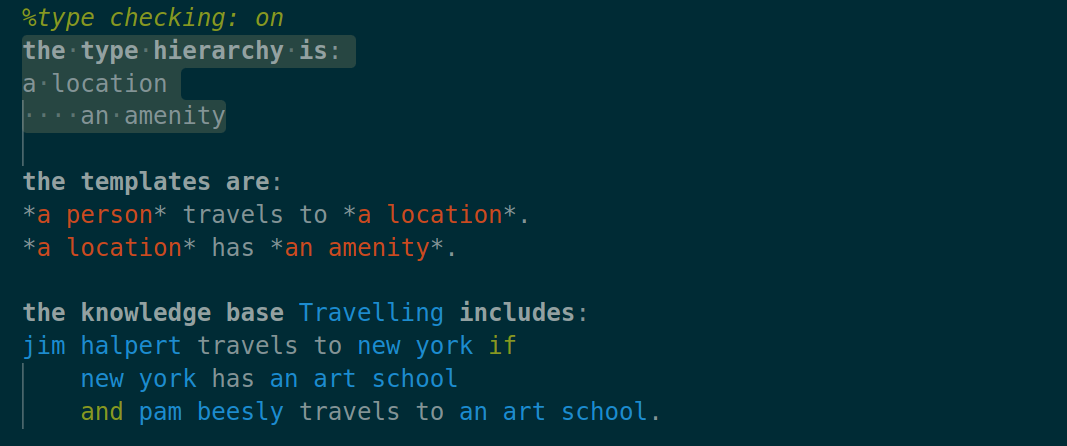
\includegraphics[width = \linewidth]{figures/type-hierarchy.png}
\caption{A type hierarchy is used to resolve the type mismatch errors shown in Figure \ref{fig:type-mismatch-2}.}
\label{fig:type-hierarchy}
\end{figure}
%
%
% \begin{figure}[h!]
% \centering

% \end{figure}
The title \codeword{the type hierarchy is:} marks the optional section where a type hierarchy can be written. To write that the type $B$ is a subtype of the type $A$, the type name of $B$ is written below the type name of $A$, indented further than $A$ by a single tab. 
\\
\\
The editor uses this type hierarchy in checking for type errors. Figures \ref{fig:type-mismatch-2} and \ref{fig:type-hierarchy} show this in action with the introduction of the template 
\begin{lstlisting}[language={LE}]
    *a driver* offers *a passenger* a lift to *a resort*.
\end{lstlisting}
As shown in Figure \ref{fig:type-mismatch-2}, when writing an atomic formula that matches the above template, supplying terms that are of type \codeword{a person} as the first two arguments causes a type mismatch error. The error is resolved in Figure \ref{fig:type-hierarchy} by introducing a type hierarchy that states that \codeword{a driver} and \codeword{a passenger} are two subtypes of the type \codeword{a person}.
\end{document}